%========================================================
% File:         TempCSMIO2018.tex
% By:           template Resúmenes CSMIO 2018
%========================================================

\documentclass[spanish,letterpaper,12pt]{article}

\usepackage{anysize}
\marginsize{2cm}{2cm}{2cm}{2cm}% izq der arriba%

\usepackage[spanish,es-tabla]{babel}
\usepackage[utf8]{inputenc}
\usepackage[numbers]{natbib}
\usepackage{graphicx}
\usepackage{caption, subcaption}
\captionsetup{labelfont = {sf,bf}}

\usepackage{amsmath}
\usepackage{amsfonts}
\decimalpoint
\renewcommand{\spanishtablename}{Cuadro}
%
% Paquetes adicionales requeridos
%
%
%  Title definition
%
%  Título, autores, adscripciones, correo electrónico
%
\title{\bf Preparaci\'on de galletas de mantequilla}

\author{Erick Cervantes--Mendieta \\
\normalsize{Posgrado en Ingenier\'ia de Sistemas, Universidad Aut\'onoma de Nuevo Le\'on,} \\
\normalsize{San Nicol\'as de los Garza, Nuevo Le\'on, M\'exico} \\
\normalsize{erick.cervantesmnd@uanl.edu.mx}
}

\date{\empty}

%
%  El documento comienza aquí
%
\begin{document}


\pagestyle{empty}

\maketitle

\begin{abstract}

En general, la formulación de una galleta consta de tres ingredientes fundamentales: harina, azúcar y grasa, en esta investigación se pretende observar el comportamiento de dos tipos de harina y cinco tipos de endulzantes para preparar galletas de mantequilla y ver si hay algún tipo de interacción entre estos que afecte el peso de las galletas mediante la implementación de un diseño de experimentos de dos factores. Dicha implementación indica que uno de los factores afecta a la variable de respuesta.

\end{abstract}

\vspace{1em}
\noindent\textit{Palabras clave:}
DOE;
galletas de mantequilla;
endulzantes;
harina de almendras.

\thispagestyle{empty}


%
%   Introduccion
%
\section{Introducci\'on}
\label{intro}

Según la norma NMX-F-006-1983, las \textbf{galletas} son el producto elaborado con harinas de trigo, avena, centeno, harinas integrales, azúcares, grasa vegetal y/o aceites vegetales comestibles, agentes leudantes, sal yodatada; adicionados o no de otros ingredientes (leche descremada en polvo, queso, suero de leche, caseinato de sodio, mantequilla o grasa butirica, huevo fresco, congelado o en polvo, frutas en sus distintas formas, mermeladas, jaleas, gomas, grenetina, agar--agar, pectinas o albuminas, chocolate y coco rayado) y aditivos alimenticios permitidos (lecitina, saboreadores, colorantes, emulsificantes, antioxidantes y mejoradores de masa autorizados por la Secretaria de Salubridad y Asistencia) los que se someten a un proceso de amasado, moldeado y horneado.\\

En dicha Norma, las \emph{galletas} se clasifica en tres tipos y un sólo grado de calidad cada uno: Tipo I (galletas finas), Tipo II (galletas entrefinas) y Tipo III (galletas comerciales). Estas últimas son las que se abordan en esta investigación, ya que se desea saber si algunos de los ingredientes principales en la preparación de galletas de mantequilla, afectan algunas de sus características, en particular, estamos interesados en el \textbf{peso} de la galleta.\\

Algunas investigaciones, en su mayoría tesis para obtención de grado, han abordado esta problemática, en la cual se desea obtener los niveles óptimos de aquellos factores que afectan en el proceso de preparación de las galletas, por ejemplo, \citet{arevalo2011} indican en su investigación que las características nutricionales de las galletas de harina de trigo se pueden mejorar mediante la adición de harina de haba  y de panela como edulcorante mediante el uso de un diseño de experimentos.\\

Una galleta hecha con un porcentaje de harina de plátano y harina de trigo para mejorar las condiciones nutricionales fue planteada por \citet{loaiza2017}, en dónde se utilizó un diseño experimental utilizando tres factores: mezcla de harinas, porcentaje de grasa y porcentaje de agua a utilizar. Otro diseño experimental de tres factores es presentado por \citet{cardenas2015}, en el cuál se consideran como factores al azúcar, la harina y la grasa (margarina), utilizando dos niveles en cada uno de ellos (alto y bajo) con \emph{una} réplica, para estudiar el comportamiento de las propiedades macroscópicas, microscópicas y moleculares de las galletas antes y después de ser horneadas.\\

La metodología Taguchi fue implementada por \citet{villarroel2009}, utilizando cuatro factores con tres niveles cada uno, para preparar galletas a base de harina desgrasada de avellana chilena y harina de quinoa, con la finalidad de incrementar las opciones nutricionales de la población.\\

Un análisis sensorial es abordado por \citet{martinez2016}, en el cuál se desea obtener una galleta con un porcentaje del $20\%$ de harina de quínoa y diferentes edulcorantes como son la tagatosa y la estevia para el mercado de pacientes diabéticos, está técnica es muy eficaz, cuando se desea saber las preferencias de alguna población en particular.\\

Nótese que en la mayoría de los trabajos citados se pretende determinar los niveles óptimos para los diferentes factores en estudio, con la finalidad de poder producir una galleta con la calidad deseada, ya sea para un público en general o para un público en particular. En esta investigación, se pretende observar si el tipo de harina y edulcorante a utilizar afecta el \emph{peso} (en gramos) de una galleta de mantequilla, mediante la implementación de un diseño de experimentos de dos factores, con la finalidad de poder obtener una galleta baja en calorías, al utilizar harina de almendras y harina de trigo integral.\\

El resto del artículo está organizado de la siguiente manera. Discutimos los materiales y la metodología utilizada en la Sección 2. En la Sección 3, se presentan los resultados y la discusión de estos y en la Sección 4, se presentan las conclusiones.


\section{Materiales y método}
\label{sec:desc}

Para elaborar aproximadamente 20 galletas de mantequilla se necesitan los siguientes ingredientes: 450 gramos de mantequilla, 2 huevos, 4 cucharadas de vainilla, 300 gramos de endulzante y 900 gramos de harina. El procedimiento se describe a continuación: se bate la mantequilla hasta obtener una consistencia cremosa, se añade los dos huevos y se sigue batiendo, luego se añade el endulzante y se integra por completo a la mezcla, finalmente se agrega la harina y se bate hasta obtener una masa con consistencia homogénea.\\

Con un rodillo se extiende la masa, la cual debe tener un mismo grosor (en nuestro caso fue de 6 mm), luego se corta la masa en figuras y se pone en una charola para llevarlas al horno precalentado a $180^\circ$, después de 15 minutos se sacan del horno y se dejan reposar.\\

Cuando hablamos de harina, nos referimos que en nuestro caso se tienen dos tipos: harina de almendras y harina de trigo  integral (ver figura \ref{f1}); de igual forma, cuando hablamos de endulzante, se tiene que puede ser: azúcar glass, azúcar morena, panela, stevia y/o splenda (ver figura \ref{f2}).
\begin{figure}[]
\begin{center}
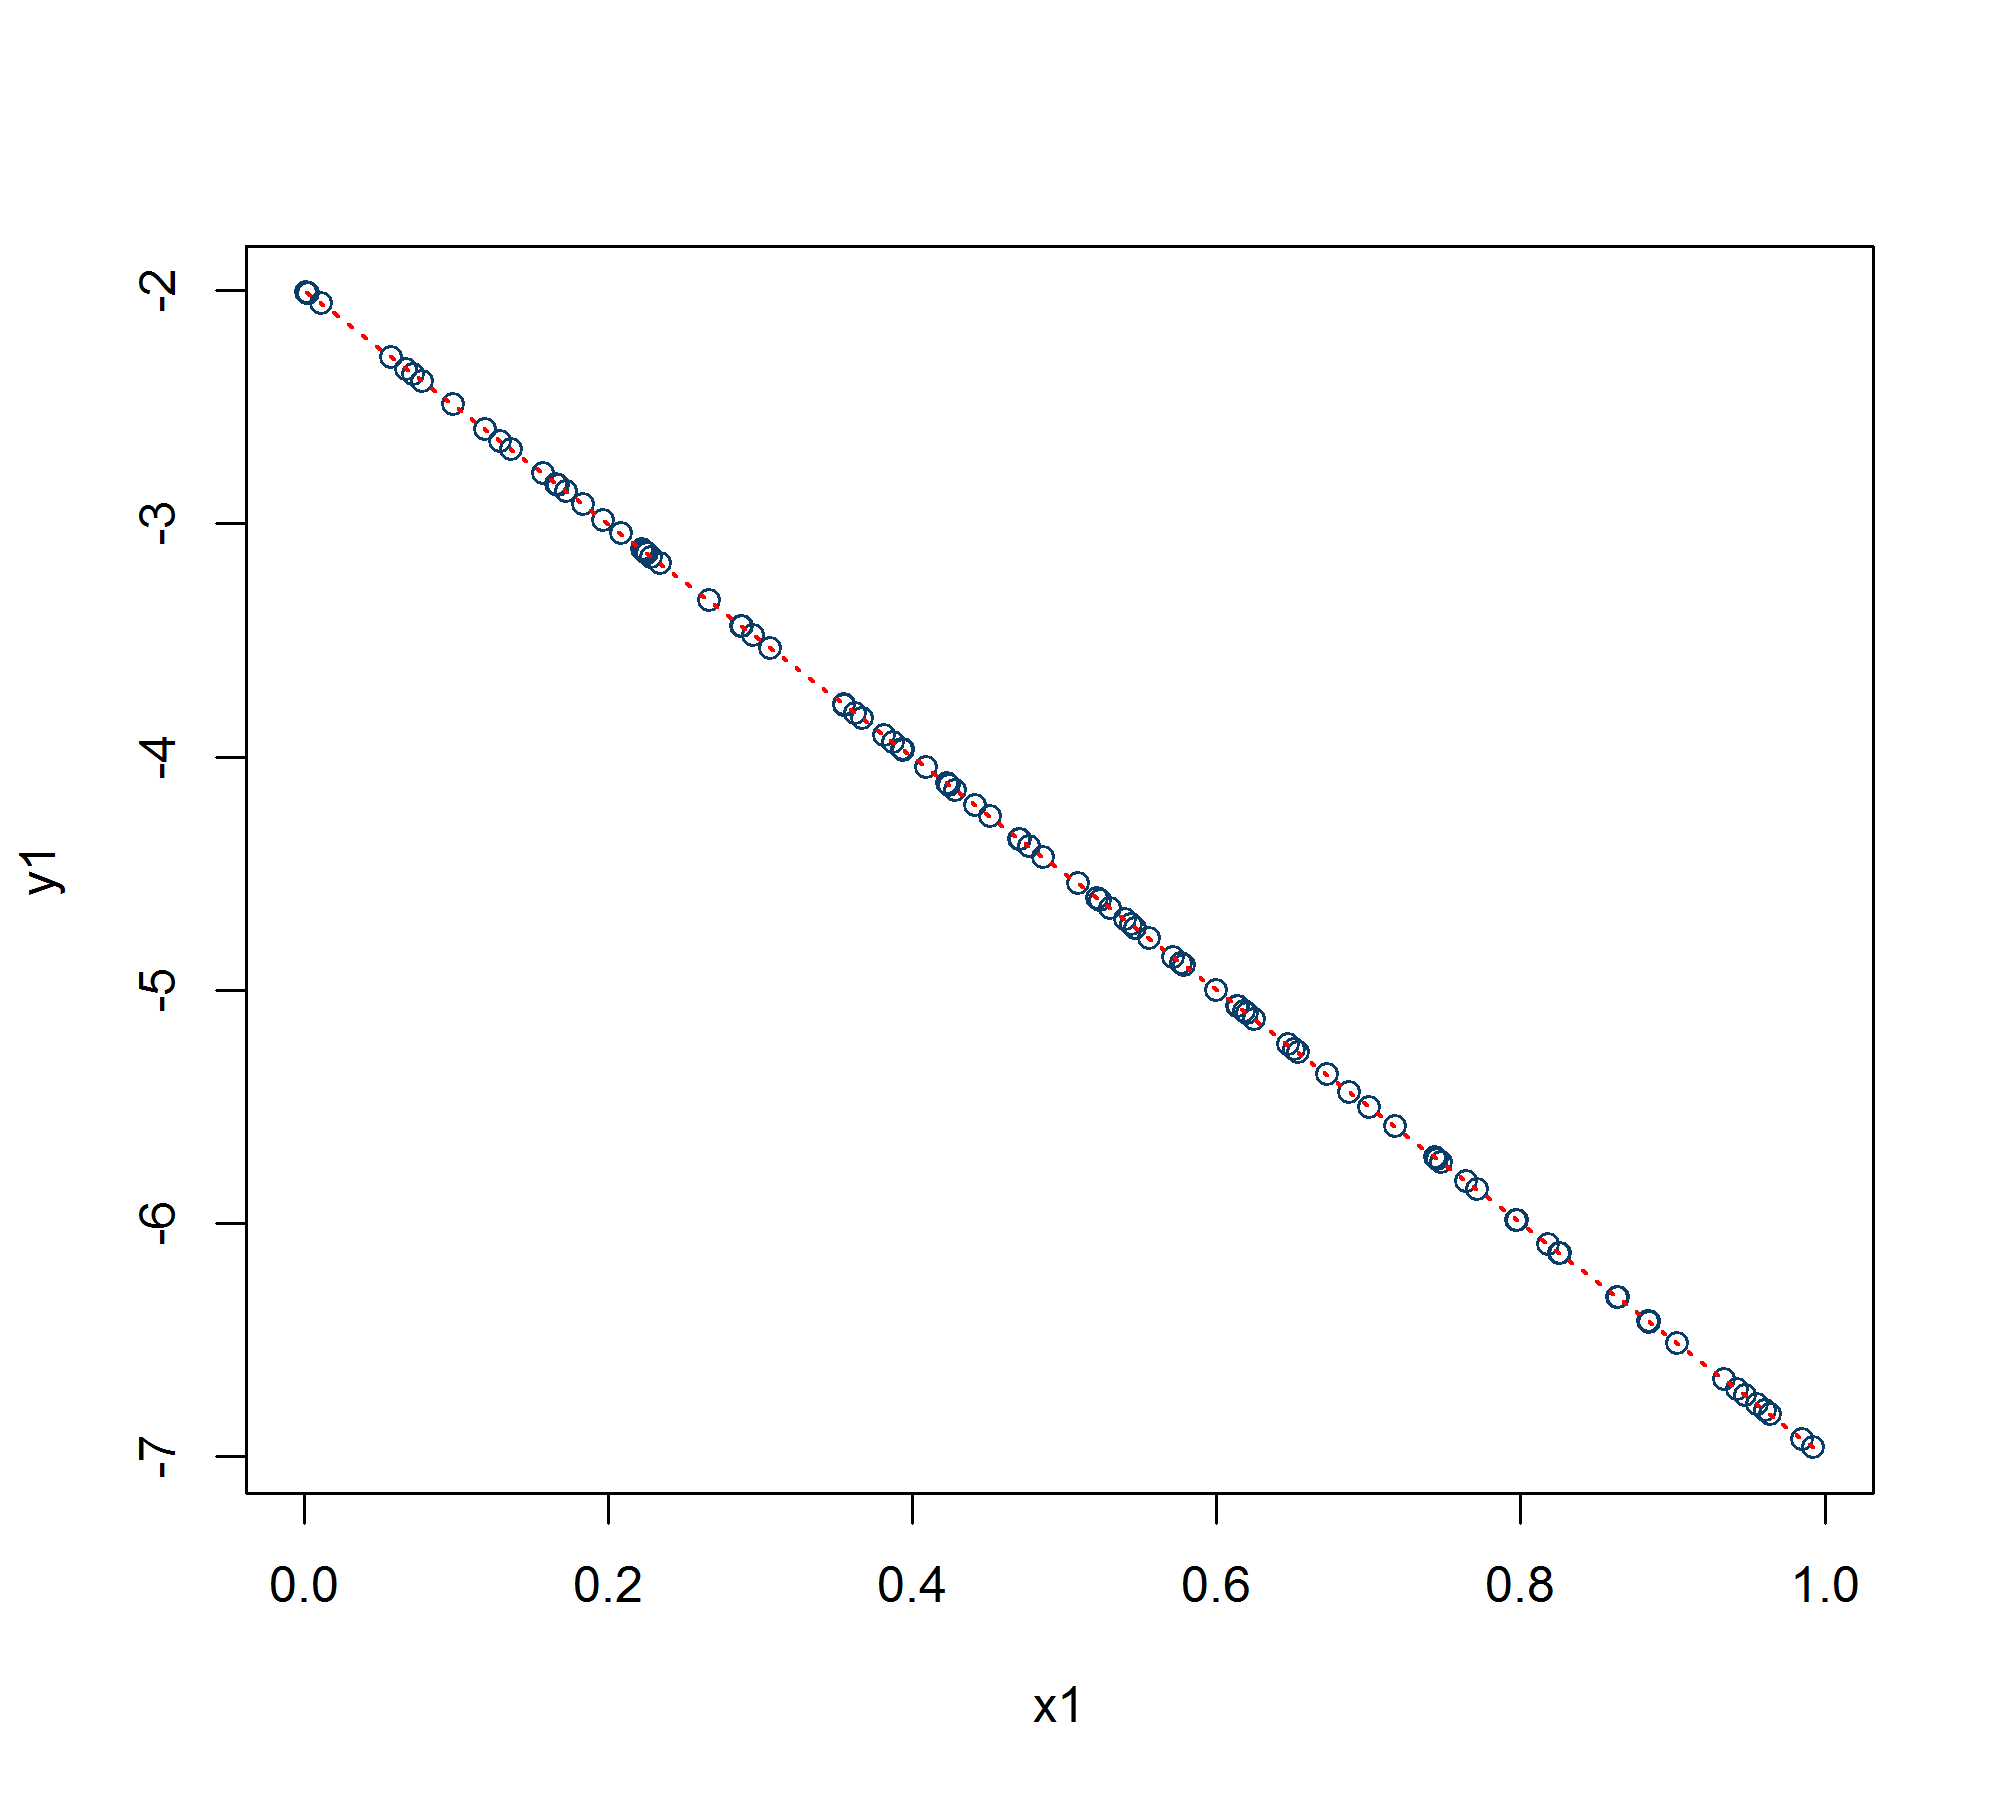
\includegraphics[width=12 cm]{Fig/f1.jpg}
\caption{Tipos de harina para hacer una galleta de mantequilla.}\label{f1}
\end{center}
\end{figure}

\begin{figure}[]
\begin{center}
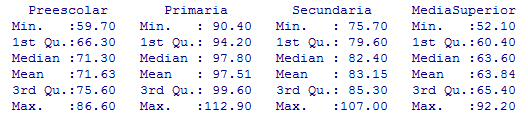
\includegraphics[width=12 cm]{Fig/f2.jpg}
\caption{Tipos de edulzantes para hacer una galleta de mantequilla.}\label{f2}
\end{center}
\end{figure}

\subsection{Diseño de experimentos}
\label{subsec:diseno}

En estadística, un \emph{experimento factorial} completo es un experimento cuyo diseño consta de dos o más factores, cada uno de ellos con distintos niveles, cuyas unidades experimentales cubren todas las posibles combinaciones de esos niveles en todo los factores, por ejemplo, si el factor $A$ tiene $a$ niveles y el factor $B$ tiene $b$ niveles, cada réplica contiene todas las $ab$ combinaciones de los tratamientos. Este tipo de experimentos permiten el estudio del efecto de cada factor sobre la \emph{variable respuesta}, así como el efecto de las \emph{interacciones} entre factores sobre dicha variable.\\

Los diseños factoriales más simples son los que incluyen únicamente dos factores o conjunto de tratamientos, por lo que si $A$ y $B$ son los factores, entonces podemos considerar que hay $a$ niveles del factor $A$ y $b$ niveles del factor $B$, y puede haber $n$ réplicas en cada uno de los tratamientos.\\

En nuestro problema consideramos el factor $A$ como el tipo de harina a utilizar con dos niveles: harina de almendras y harina de trigo; al factor $B$ como el tipo de edulzante, con 5 niveles: azúcar glass, azúcar morena, panela, stevia y splenda. En el Cuadro \ref{cuadro1} se presentan los datos del experimento y el peso observado de cada galleta, notése que solo se tiene una réplica, por lo que el análisis de varianza (ANOVA) para esta situación se puede visualizar en el Cuadro \ref{cuadro2}. Una prueba desarrollada por Tukey (\citet{montgomery2003}) es útil para determinar si está presente una interacción, en dicha prueba se hace la partición de la suma de cuadrados de los residuales en un componente con un solo grado de libertad debido a la no aditividad (\emph{interacción}) y un componente del error con $(a-1)(b-1)-1$ grados de libertad. Así, se deberá calcular lo siguiente:
\begin{equation*}
  SS_N = \frac{\left[\sum_{i=1}^{a} \sum_{j=1}^{b} y_{ij}y_{i.}y_{.j} - y_{..}\left(SS_A + SS_B + \frac{y^2_{..}}{ab}\right)\right]^2}{abSS_A SS_B}
\end{equation*}
\noindent con un grado de libertad, y $SS_{Error} = SS_{Residual} - SS_N$ con $(a-1)(b-1)-1$ grados de libertad. Para probar la presencia de una interacción, se calcula
\begin{equation*}
  F_0 = \frac{SS_N}{SS_{Error} / [(a-1)(b-1)-1]}
\end{equation*}
\noindent si $F_0 > F_{\alpha,1,(a-1)(b-1)-1}$, debe \emph{rechazarse la hipótesis de que no hay ninguna interacción}.

\begin{table}[]
\begin{center}
  \caption{Datos para el peso de las galletas y los diferentes tratamientos que se utilizaron.}
\begin{tabular}{c|ccccc}
                                  & \multicolumn{5}{c}{\textit{\textbf{Tipo de endulzante}}}                                              \\
\textit{\textbf{Tipo de harina}}  & \textbf{Stevia} & \textbf{Azúcar glass} & \textbf{Splenda} & \textbf{Azúcar morena} & \textbf{Panela} \\
\hline
\textbf{Harina de almendras}      & 18              & 18                    & 18               & 19                     & 18              \\
\textbf{Harina de trigo integral} & 20              & 20                    & 19               & 19                     & 18
\end{tabular}
\label{cuadro1}
\end{center}
\end{table}

\begin{table}[]
\begin{center}
  \caption{Análisis de varianza de un modelo de dos factores, una observación por celda.}
\begin{tabular}{ccccc}
\begin{tabular}[c]{@{}c@{}}Fuente de\\ variación\end{tabular} & \begin{tabular}[c]{@{}l@{}}Suma de\\ cuadrados\end{tabular} & \begin{tabular}[c]{@{}c@{}}Grados de\\ libertad\end{tabular} & \begin{tabular}[c]{@{}l@{}}Cuadrado\\ medio\end{tabular} & \begin{tabular}[c]{@{}c@{}}Cuadrado medio\\ esperado\end{tabular} \\
\hline
Renglones ($A$) & $\sum^{a}_{i=1} \frac{y^2_{i.}}{b} - \frac{y^2_{..}}{ab}$ & $a-1$ & $MS_A$ & $\sigma^2+\frac{b\sum\tau^2_i}{a-1}$ \\
Columnas ($B$) & $\sum^{b}_{j=1} \frac{y^2_{.j}}{a} - \frac{y^2_{..}}{ab}$ & $b-1$ & $MS_B$ & $\sigma^2+\frac{a\sum\beta^2_j}{b-1}$ \\
Residual o $AB$ & Sustracción & $(a-1)(b-1)$ & $MS_{Residual}$ & $\sigma^2+\frac{\sum\sum(\tau \beta)^2_{ij}}{(a-1)(b-1)}$ \\
Total & $\sum_{i=1}^{a} \sum_{j=1}^{b} y^2_{ij} - \frac{y^2_{..}}{ab}$ & $ab-1$ & & \\
\hline
\end{tabular}
\label{cuadro2}
\end{center}
\end{table}

\section{Resultados y análisis}
\label{sec:metodo}

Con la ayuda del lenguaje R \nocite{LenguajeR} se pueden obtener algunos valores para la tabla ANOVA, pero algunos valores deben calcularse de manera manual. Luego, se sigue que:
\begin{equation*}
  SS_A = \frac{1}{5} \left[91^2 + 96^2\right] - \frac{187^2}{(2)(5)} = 2.5,
\end{equation*}
\begin{equation*}
  SS_B = \frac{1}{2} \left[38^2 + 38^2 + 37^2 + 38^2 + 36^2\right] - \frac{187^2}{(2)(5)} = 1.6,
\end{equation*}
\begin{equation*}
  SS_T = 18^2 + 18^2 + \ldots + 19^2 + 18^2 - \frac{187^2}{(2)(5)} = 3503 - 3496.9 = 6.1,
\end{equation*}
\begin{equation*}
  SS_{Residual} = 6.1 - 2.5 - 1.6 = 2,
\end{equation*}
\begin{equation*}
  \sum_{i=1}^{a} \sum_{j=1}^{b} y_{ij} y_{i.} y_{.j} = (18)(91)(38) + (18)(91)(38) + \ldots + (18)(96)(36) = 654692,
\end{equation*}
\begin{equation*}
  SS_N = \frac{[654692 - 187(2.5 + 1.6 + 3496.9)]^2}{(2)(5)(2.5)(1.6)} = 0.625,
\end{equation*}
\begin{equation*}
  SS_{Error} = SS_{Residual} - SS_N = 2 - 0.625 = 1.375.
\end{equation*}

El análisis de varianza completo se resume en el Cuadro \ref{cuadro3}, en dónde, se observa que el estadístico de prueba para la no aditividad es $F_0 = 0.733$ con $F_{0.05,1,3} = 10.13$, por lo que no hay evidencia de interacción en los datos entre los dos factores. Para los efectos principales de tipo de harina y tipo de endulzante son $F_{0.05,1,4} = 7.71$ y $F_{0.05,4,4} = 6.39$, respectivamente.

\begin{table}[]
\begin{center}
  \caption{ANOVA para el problema de la preparación de galletas de mantequilla.}
\begin{tabular}{ccccc}
\textbf{\begin{tabular}[c]{@{}c@{}}Fuente de\\ variación\end{tabular}} & \textbf{\begin{tabular}[c]{@{}c@{}}Suma de\\ cuadrados\end{tabular}} & \textbf{\begin{tabular}[c]{@{}c@{}}Grados de\\ libertad\end{tabular}} & \textbf{\begin{tabular}[c]{@{}c@{}}Cuadrado\\ medio\end{tabular}} & \textbf{$F_0$} \\
\textbf{Harina}                                                        & 2.5                                                                  & 1                                                                     & 2.5                                                               & 5.45          \\
\textbf{Endulzante}                                                    & 1.6                                                                  & 4                                                                     & 0.4                                                               & 0.873         \\
\textbf{No aditividad}                                                 & 0.625                                                                & 1                                                                     & 0.625                                                             & 0.733         \\
\textbf{Error}                                                         & 1.375                                                                & 3                                                                     & 0.458                                                             &               \\
\textbf{Total}                                                         & 6.1                                                                  & 9                                                                     &                                                                   &
\end{tabular}
\label{cuadro3}
\end{center}
\end{table}

%   Conclusiones
%
\section{Conclusiones}
\label{conclusiones}

El diseño de experimentos de dos factores permitió visualizar que los dos factores escogidos no tienen interacción alguna entre ellos para afectar el peso de las galletas de mantequilla, sin embargo, se encontró que el peso de la galleta si se ve afectado por el tipo de edulzante que se utiliza, mientras que para el tipo de harina no hay evidencia de que afecte en el peso de la galleta.\\

Hace falta un análisis más detallado para poder analizar otras características de las galletas como lo es, el sabor, la textura y la aceptabilidad de algún público en particular, que desee consumir este tipo de galleta baja en calorías.

\section{Trabajo futuro}

Se desea implementar un análisis sensorial para poder determinar si las galletas son o no del agrado de las personas, para poder encontrar los niveles de los factores que permitan producir galletas que llamen la atención para su venta.

%
%   Referencias
%
%\bibliographystyle{plainnat}
\bibliographystyle{apa}
\bibliography{ProbBiblio}


\end{document}

